\def\VCDate{2016/02/12}\def\VCVersion{(Current)}
\documentclass{article}
\usepackage[screen]{geometry}
\usepackage{ProofPower, verbatim, graphicx, color, amsmath, amssymb}
\begin{document}
\underscoreoff

\title{CS118 Lab:1}
\author{Saw Thinkar Nay Htoo}
\maketitle


\section*{Choosing a car}
An algorithm is described to help select the best car based on overall cost related to fuel efficiency.
\begin{description}
\item[Inputs:] : purchase price and fuel efficiency (in mpg)
\item[Process:] :\\
total cost = purchase price + operating cost \\
operating cost = years times annual fuel cost \\
anuual fuel cost = price per gallon times the annual fuel consumed. 
\item[Output:] total cost
\end{description}
\section*{analysis}
Assuming (since the specification does not indicate it), the number of years will be 10. And then, if the inputs are 15,000 miles per year and gas costs \$3 per gallon. And the inputs are purchase price of \$25,000 and fuel efficiency is 45mpg. 
\begin{description}
\item[Inputs:] : purchase price and fuel efficiency (in mpg)
\item[Process:] :\\
total cost = 25000 + operating cost \\
operating cost = 10 times annual fuel cost \\
annual fuel cost = 3 times 15000/45.
\item[Output:] total cost
\end{description}
\clearpage
\section*{prototype SML code}
\begin{GFT}{SML}
\+fun annual\_fuel\_consumed(ppg,mpy,mpg) = ppg*mpy div mpg;\\
\+val ppg = 3; val mpy = 15000; val mpg = 45;\\
\+val fuel = annual\_fuel\_consumed(ppg,mpy,mpg);\\
\+val years = 10;\\
\+fun operating\_cost(fc) = years * fc;\\
\+val cost = operating\_cost(fuel);\\
\+val pp = 25000;\\
\+fun total\_cost(oc) = pp + oc;\\
\+val total = total\_cost(cost);\\
\end{GFT}
\clearpage
\section*{Output from SML code}
\verbatiminput{result}

\clearpage
\section*{C code implementation of the SML code}
\begin{GFT}{Text written to file lab1.c}
\+\#include <stdio.h>\\
\+\\
\+int eax = 0;\\
\+\\
\+int annual\_fuel\_consumed(int ppg, int mpy, int mpg)\\
\+	\{return ppg * mpy/mpg;\}\\
\+int fuel; int cost; int total;\\
\+\\
\+\#define years 10\\
\+int operating\_cost(int fc) \{ return years * fc; \}\\
\+\#define pp 25000\\
\+int total\_cost(int oc) \{ return pp + oc; \}\\
\+\\
\+\#define ppg 3\\
\+\#define mpy 15000\\
\+\#define mpg 45\\
\+int fuel; int cost; int total;\\
\end{GFT}
\clearpage
The output when running C program.
\begin{GFT}{Text appended to file lab.c}
\+int main()\\
\+\{\\
\+	fuel = annual\_fuel\_consumed(ppg,mpy,mpg);\\
\+	cost = operating\_cost(fuel);\\
\+	total = total\_cost(cost);\\
\+	printf("Total cost of car: \%i\Backslash{}n",total);\\
\+\}\\
\+\Backslash{}clearpage\\
\+\Backslash{}section*\{C code implementation of the SML code\}\\
\end{GFT}
\begin{GFT}{Text written to file lab.c}
\+\#include <stdio.h>\\
\+int eax; int ebx; int ecx;\\
\+int fuel; int cost; int total;\\
\+\\
\+//int annual\_fuel\_consumed(int ppg,int mpy,int mpg)\\
\+//\{return ppg* mpy/mpg;\}\\
\+\\
\+void annual\_fuel\_consumed2()\\
\+\{eax = eax * ebx / ecx;\}\\
\+\\
\+\#define years 10\\
\+int operating\_cost(int fc) \{return years * fc;\}\\
\+void operating\_cost2() \{eax = years * eax;\}\\
\+\#define pp 25000\\
\+int total\_cost(int oc) \{return pp + oc;\}\\
\+int total\_cost2() \{return pp+ eax;\}\\
\+\#define ppg 3\\
\+\#define mpy 15000\\
\+\#define mpg 45\\
\+int main()\\
\+\{\\
\+	//fuel = annual\_fuel\_consumed(ppg,mpy,mpg);\\
\+	eax = ppg;\\
\+	ebx = mpy;\\
\+	ecx = mpg;\\
\+	fuel = annual\_fuel\_consumed2();\\
\+	//cost = operating\_cost(fuel);\\
\+	eax = fuel;\\
\+	//cost = operating\_cost2();\\
\+	operating\_cost2(); //assume return value is in eax\\
\+	//cost = eax;\\
\+	//total = total\_cost(cost);\\
\+	//eax = cost;\\
\+	total = total\_cost2();\\
\+	printf("Total cost of car: \%i\Backslash{}n",total);\\
\+	return 0;\\
\+\}\\
\end{GFT}
The output when running the C program in the debugger is: 

\begin{center}
	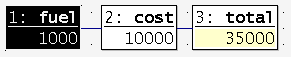
\includegraphics{out1.png}
\end{center}

\clearpage
\section*{Translation of C code to ASM code}
\begin{itemize}
\item include statements (libraries like stdio)
\item declare variables
\item define functions
\item symbolic constants (in C define) \\
e.g. \verb|#define x 0 in C would be \verb|.equ x,0 in asm
\item assignment statements
\item call assembly language functions
\item call C functions (printf) \\
e.g. the call to printf: printf("Total cost of car: %i\n",total); in asm is:
\begin{verbatim}  
  push %eax\\
  push $msg\\
  call printf\\
  add $8,%esp\\
\end{verbatim}
\item return from main function 
\item arithmetic operations (addition, multiplication, integer division)
\end{itemize}
\begin{GFT}{Text written to file lab1.s}
\+.equ ppg,3\\
\+.equ mpy,15000\\
\+.equ mpg,45\\
\+.data\\
\+  fuel: .long 0\\
\+  total: .long 0\\
\+  cost: .long 0\\
\+msg: .string "fuel: \%i\Backslash{}n"\\
\+.text\\
\+ annual\_fuel\_consumed:\\
\+  mov \$ppg,\%eax\\
\+  mov \$mpy,\%ebx\\
\+  mul \%ebx \# edx:eax = eax * ebx\\
\+  mov \$mpg, \%ecx\\
\+  div \%ecx \# eax = edx:eax / ecx\\
\+\\
\+  push \%eax\\
\+  push \$msg\\
\+  call printf\\
\+  add \$8,\%esp\\
\+  \\
\+ ret\\
\+ .globl main\\
\+main:\\
\+ call annual\_fuel\_consumed\\
\+ ret\\
\+\\
\+\\
\end{GFT}
\clearpage
\section*{Shell scripts to make processing easier}
This shell script is used to make extracting and processing the source code easier. The -g option to the gcc compiler adds debugging symbols so we can refer to variables even though they are not normally stored in the object code. 
\begin{GFT}{Text written to file labcode.sh}
\+docsml lab1.doc\\
\+gcc -Wall -g -o lab1c lab1.c\\
\end{GFT}
\begin{GFT}{Text written to file labdoc.sh}
\+doctex lab1.doc\\
\+pptexenv pdflatex lab1.tex\\
\end{GFT}
\begin{GFT}{Bourne Shell}
\+chmod 755 labcode.sh\\
\+chmod 755 labdoc.sh\\
\+\\
\+poly < lab1.sml > result\\
\end{GFT}

\end{document}
